\documentclass[12pt]{article}
\usepackage[a4paper,total={6in,9in}]{geometry}
\usepackage{wrapfig}
\usepackage{graphicx}
\usepackage{amssymb}
\usepackage{mathtools}
\usepackage{listings}
\usepackage{url}
\usepackage{hyperref}
\usepackage{xcolor}

\author{\textbf{Rahul Girotra} \\ \textbf{2018JTM2246}\\ \textbf{2018-19}}
\date{}
\title{\textbf{Assignment-8\\ELP- 718 Telecom Software Laboratory}}

\begin{document} 
	\maketitle
	
	\begin{center}
	\noindent \textbf{A report presented for the assignment on\\ Python/Github}
	\vspace{1cm}
	
	\begin{figure}[h]
	\centering
	
\includegraphics[scale=.2]{iitd.jpg}
	
	
	\end{figure}
	\vspace{1.5cm}
	
	\textbf{Bharti School\\of\\Telecommunication Technology and Management\\IIT DELHI, Delhi\\September 27, 2018}
	
	\end{center}
	
	\newpage
	\tableofcontents
	\listoffigures
	\newpage
	
	\section{Problem Statement-1}
	
	
		\subsection{Problem Statement}\cite{problem1}
			IIT Delhi, has just got the strongest computer. The professors in charge wants to check the computational capacity of the computer. So, they decided to create the problem which is to be given as an assignment to students. Can you help the professor to check the computation capability of the computer?
		A valid cross is defined here as the two regions (horizontal and vertical) of equal lengths crossing over each other. These lengths must be odd, and the middle cell of its horizontal region must cross the middle cell of its vertical region.

			\begin{figure}
			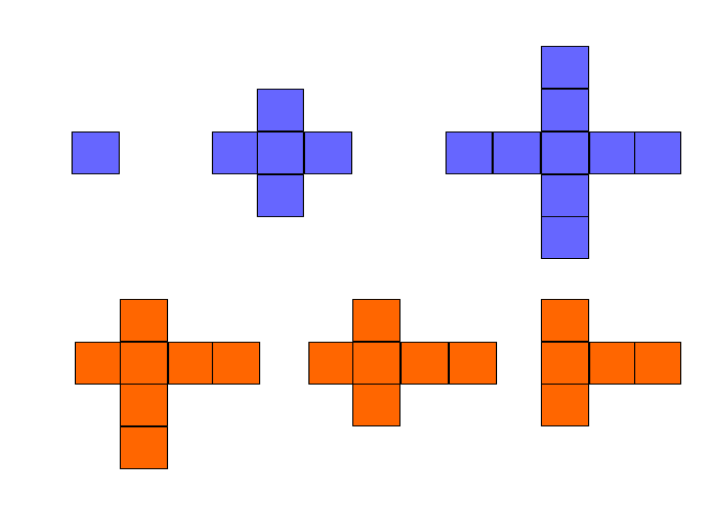
\includegraphics[scale=0.6]{ps1p1.png}
			\end{figure}
		\subsection{Assumptions}
		
			\begin{itemize}
				\item $$2 <= n <= 105$$
				\item $$2 <= m <= 105$$
			\end{itemize}
		
		\subsection{Algorithm and Implementation~\cite{}}
		
			\begin{itemize}
				\item firstly the data is made input in form of rows and coloumns.
				\item then the matrix that includes the data is inputed and printed by the user. 
			    \item correspondingly, the elements are checked by using for loop 
			    \item and corresponding data is printed accordingly. 
			 
			\end{itemize}
		
		\subsection{Flow Chart}
		
			\begin{figure}[h!]
				\centering
				\caption{Flow Chart for Figure 1}
				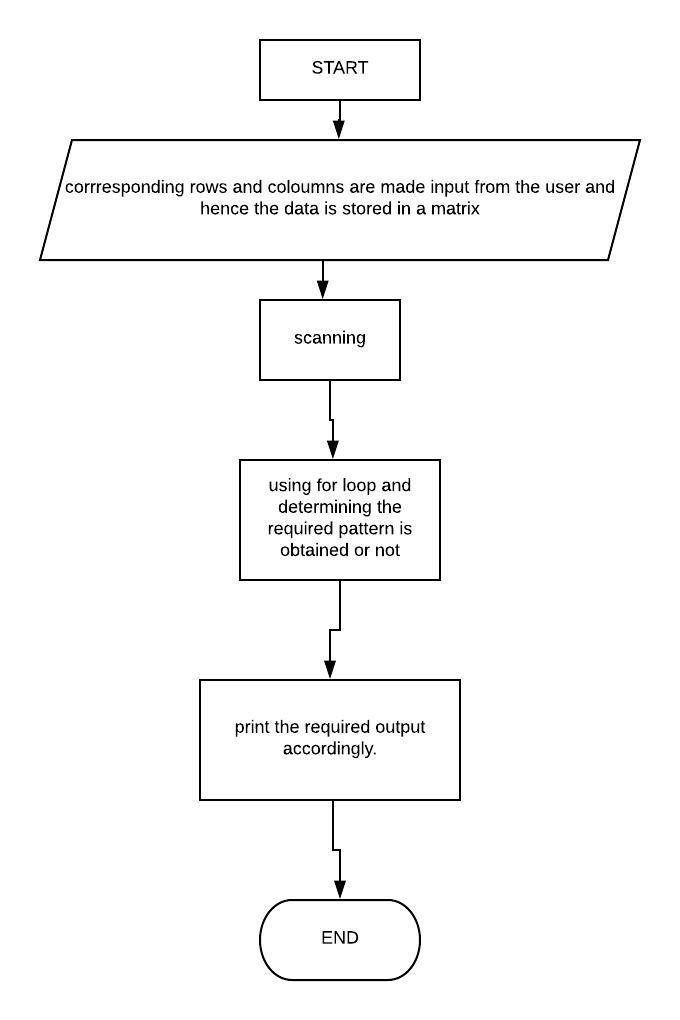
\includegraphics[scale=.8]{ps1f1.jpeg}
			\end{figure}
		
		\subsection{Input and Output Format}
		
			\begin{itemize}
				\item Input Format: The first line contains two space-separated integers,  n and m. 
Each of the next  lines n contains a string of  m characters where each character is either S (Smart) or D (Dull). These strings represent the rows of the grid. If the jth character in the ith  line is S, then  (i,j) is a  cell smart. Otherwise it's a  dull cell.
\\
				\item Output Format:Find two valid crosses that can be drawn on smart cell of the grid, and return the dimension of both the crosses in the reverse sorted order(i.e. First Dimension should be the larger one and other should be smaller one).\\ 
			\end{itemize}
		
		\subsection{Screenshots}
		
			\begin{figure}[h!]
				\centering
				\caption{Terminal Output of Problem 1}
				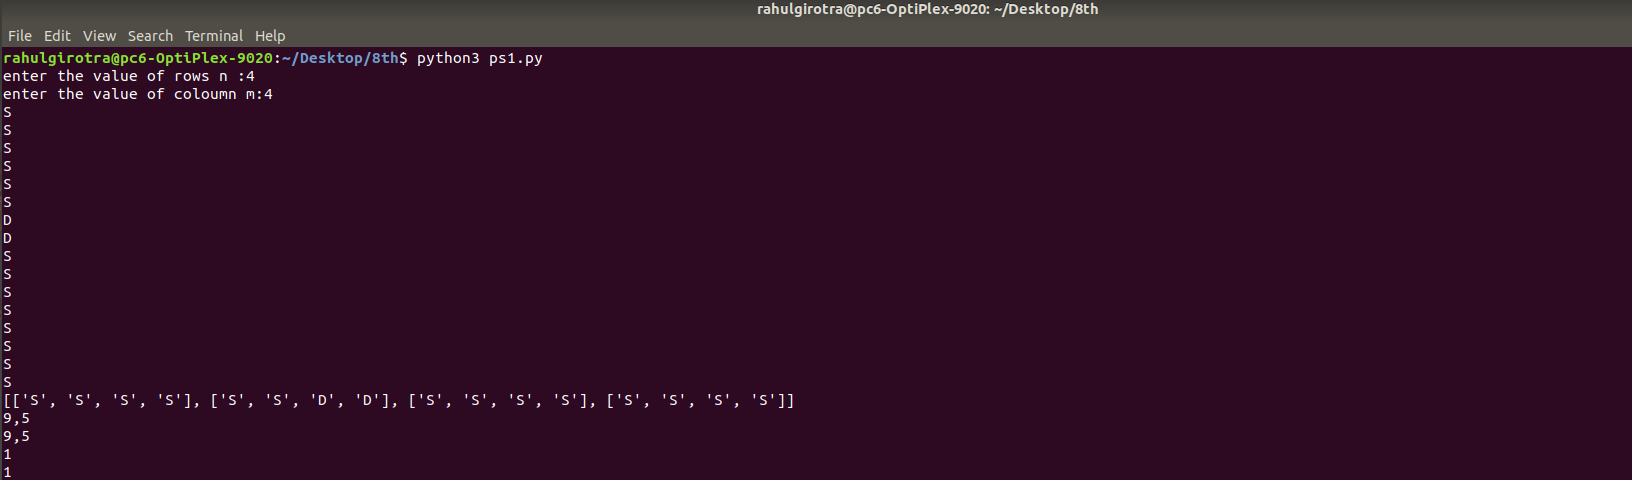
\includegraphics[scale=.5]{ps1s1.png}
			\end{figure}
	 
	\section{Problem Statement-2} \cite{problem2}
	
		\subsection{Problem Statement}
			After, getting mix results of valid crosses, professors decided to test the computation abilities on one more problem. This time professors wanted to test the decryption capabilities of the computer.
Encryption of  a message requires three keys, k1, k2, and k3. The 26 letters of English and underscore are divided in three groups,  [a-i] form one group, [j-r] a second group, and everything else ([s-z] and underscore) the third group. Within each group the letters are rotated left by ki positions in the message. Each group is rotated independently of the other two. Decrypting the message means doing a right rotation by ki positions within each group.

			
		
		
		\subsection{Assumptions}
		
			\begin{itemize}
				\item $$ 1 <= Length of the string <=150 $$

				\item $$ 1<= ki <=150 (i=1,2,3) $$
			\end{itemize}
		
		\subsection{Algorithm and Implementation~\cite{}}
		
			\begin{itemize}
			\item dividing the characters in group 1,2 and 3
			\item taking input of keys and messages
			\item dividing the characters of messages in different groups
			\item rotating and displaying the decrypted result.
			\end{itemize}
		
		\subsection{Flow Chart}
		
			\begin{figure}[h!]
				\centering
				\caption{Flow Chart of Problem 2}
				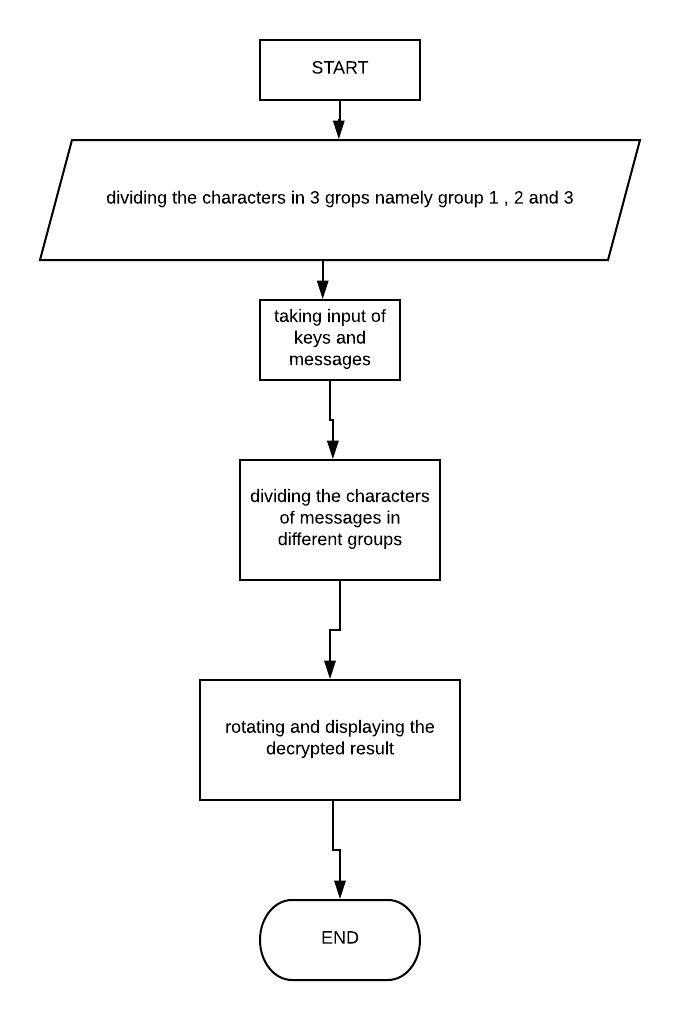
\includegraphics[scale=.8]{ps2f1.jpeg}
			\end{figure}
		
		
		\subsection{Input and Output Format}
			\textbf{Input Format:}
			\begin{itemize}
				\item All input strings comprises of only lowercase English alphabets and underscores
				
			 
			\end{itemize}
			\textbf{Output Format:}
			\begin{itemize}
				\item  For each encrypted message, the output is a single line containing the decrypted string.
				
				
			\end{itemize}
		\subsection{Screenshots}
		
			\begin{figure}[h!]
				\centering
				\caption{Terminal Output of Problem 2}
				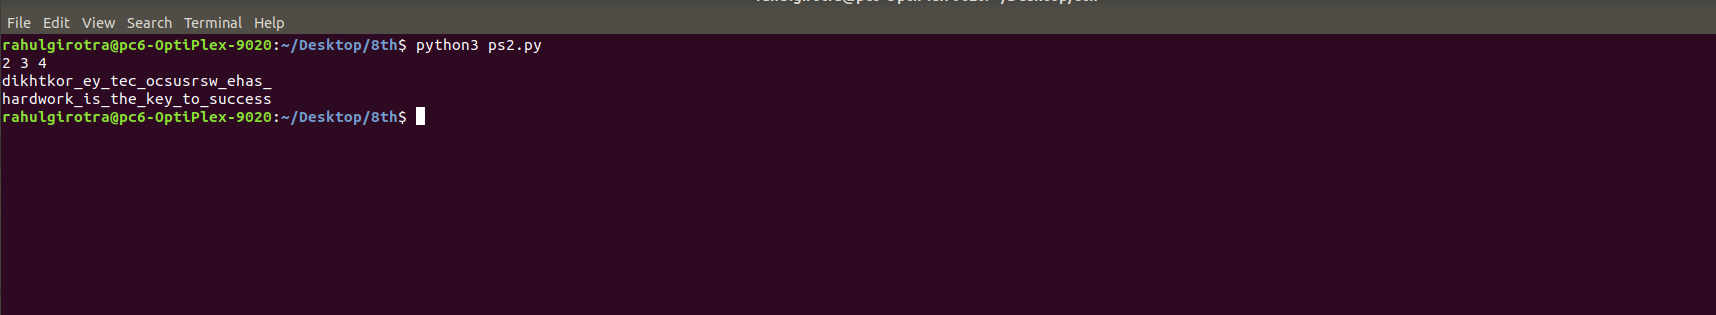
\includegraphics[scale=.5]{ps2s2.png}
			\end{figure}
		
	\section{Appendix}
	
	
		\subsection{Code for ps1}
		
			\begin{verbatim}
			n=int(input("enter the value of rows n :"))  #entering the number of rows and coloumns
m=int(input("enter the value of coloumn m:"))
matrix  = []

for i in range(0,m):       #entering the various elements of matrix from the user
	matrix.append([])
for i in range(0,n):
	for j in range(0,m):
		matrix[i].append(j)
		matrix[i][j]=0
for i in range(0,n):
	for j in range(0,m):
	 matrix[i][j] = input()
print(matrix)



for i in range(0,m):  #checking the different patterns in the matrix and accordingly printing the data
	for j in range(0,n):
		if matrix[i][j]=="S" :
			if  matrix[i-1][j]=="S" and matrix[i-2][j]=="S" and matrix[i+1][j]=="S" and matrix[i+2][j]=="S" and matrix[i][j+1]=="S" and matrix[i][j+2]=="S" and matrix[i][j-1]=="S" and matrix[i][j-2]=="S":
				print("9,5")
		
			elif  matrix[i-1][j]=="S" and matrix[i+1][j]=="S" and matrix[i][j-1]=="S" and matrix[i][j+1]=="S" :
				print("5,1")
		
		else:
			print("1")

			\end{verbatim}
			%\lstinputlisting[language]{}
		
		\subsection{Code for ps2}
		
			\begin{verbatim}
			
def rot(x1,x2):       #rot function is defined here for rotation
    copy = list(x1)
    for i in range(len(x1)):
        if x2<0:
            x1[i+x2] = copy[i]
        else:
            x1[i] = copy[i-x2]



group1="abcdefghi"   #Creating 3 groups
group2="jklmnopqr"
group3="stuvwxyz_"

gr1 =[]
gr2 =[]
gr3 =[]
gr1new=[]
gr2new=[]
gr3new=[]


a1,a2,a3 = list(map(int,input().split()))   #geting the key value from user


word = input()   #geting the string
word_list = list(word)



for i in range(0,len(word)):   #now compairing g1 in string and copy similaar char into s1
	if word_list[i] in group1:
		gr1.append(word_list[i])
		gr1new.append(i)
		
	elif word_list[i] in group2:
	    gr2.append(word_list[i])
	    gr2new.append(i)
	elif word_list[i] in group3:
	    gr3.append(word_list[i]) 
	    gr3new.append(i)




rot(gr1,a1)   #rotating  gr1,gr2,gr3 by calling rot function
rot(gr2,a2)
rot(gr3,a3)




x=y=z=0
for i in range(0,len(word)+1):     #geting back the decrypted word
	if i in gr1new:
		word_list[i]=gr1[x]
		x+=1
	elif i in gr2new:
		word_list[i]=gr2[y]
		y+=1
	elif i in gr3new:
		word_list[i]=gr3[z]
		z+=1	


for i in word_list[:]:
	print (i, end ='')

print("")
			\end{verbatim}
			%\lstinputlisting[language]{}
		
		\bibliographystyle{plain}
		\bibliography{report.bib}

\end{document}
